\documentclass[12pt]{article}
\usepackage{setspace}
\setstretch{1}
\usepackage{amsmath,amssymb, amsthm}
\usepackage{graphicx}
\usepackage{bm}
\usepackage[hang, flushmargin]{footmisc}
\usepackage[colorlinks=true]{hyperref}
\usepackage[nameinlink]{cleveref}
\usepackage{footnotebackref}
\usepackage{url}
\usepackage{listings}
\usepackage[most]{tcolorbox}
\usepackage{inconsolata}
\usepackage[papersize={8.5in,11in}, margin=1in]{geometry}
\usepackage{float}
\usepackage{caption}
\usepackage{esint}
\usepackage{url}
\usepackage{enumitem}
\usepackage{subfig}
\usepackage{wasysym}
\newcommand{\ilc}{\texttt}
\usepackage{etoolbox}
\usepackage{algorithm}
% \usepackage{algorithmic}
\usepackage[noend]{algpseudocode}
\usepackage{tikz}
\usepackage{listings}
\usepackage{color}
\usetikzlibrary{matrix,positioning,arrows.meta,arrows}
\patchcmd{\thebibliography}{\section*{\refname}}{}{}{}



\definecolor{dkgreen}{rgb}{0,0.6,0}
\definecolor{gray}{rgb}{0.5,0.5,0.5}
\definecolor{mauve}{rgb}{0.58,0,0.82}

\lstset{frame=tb,
  language=Python,
  aboveskip=3mm,
  belowskip=3mm,
  showstringspaces=false,
  columns=flexible,
  basicstyle={\small\ttfamily},
  numbers=none,
  numberstyle=\tiny\color{gray},
  keywordstyle=\color{blue},
  commentstyle=\color{dkgreen},
  stringstyle=\color{mauve},
  breaklines=true,
  breakatwhitespace=true,
  tabsize=3
}

\begin{document}

\title{\textbf{CSDS 313: Assignment 1}}

\author{Shaochen (Henry) ZHONG, \ilc{sxz517} \\Ningjia Huang, \ilc{nsh239}}
\date{Due and submitted on 08/26/2020 \\ CSDS 455, Dr. Connamacher}
\maketitle




\section*{(1)}
\begin{lstlisting}
    df = pd.read_excel('covid_data.xlsx')
\end{lstlisting}

There are \textbf{11} columns and \textbf{38283} rows in the spreadsheet.

\section*{(2)}
\begin{lstlisting}
    L = []
    i = 0
    for country in df['countriesAndTerritories']:
    if country not in L:
        L.append(country)
        print(country)
    i += 1
    print(i)
\end{lstlisting}

There are \textbf{209} countries in total.

\begin{lstlisting}
    print(df.dateRep.min())
\end{lstlisting}

The earliest date recorded is \textbf{12/31/2019}.

\begin{lstlisting}
    print(df.dateRep.max())
\end{lstlisting}

The latest date recorded is \textbf{8/24/2020}.

\section*{(3)}
\begin{lstlisting}
i = 0
countries = []
populations = []
for country in df['countriesAndTerritories']:
    if country not in countries:
        countries.append(country)
        pop = df.at[df['countriesAndTerritories'].eq(country).idxmax(),
        'popData2019'].astype('float')
        populations.append(pop)
        i += 1
df2 = pd.DataFrame({'country': countries, 'population': populations})
mean = df2['population'].mean()
print(mean)
std = df2['population'].std()
print(std)
df2['population'].hist(range = [0,200000000])
plt.show()
\end{lstlisting}

\begin{center}
    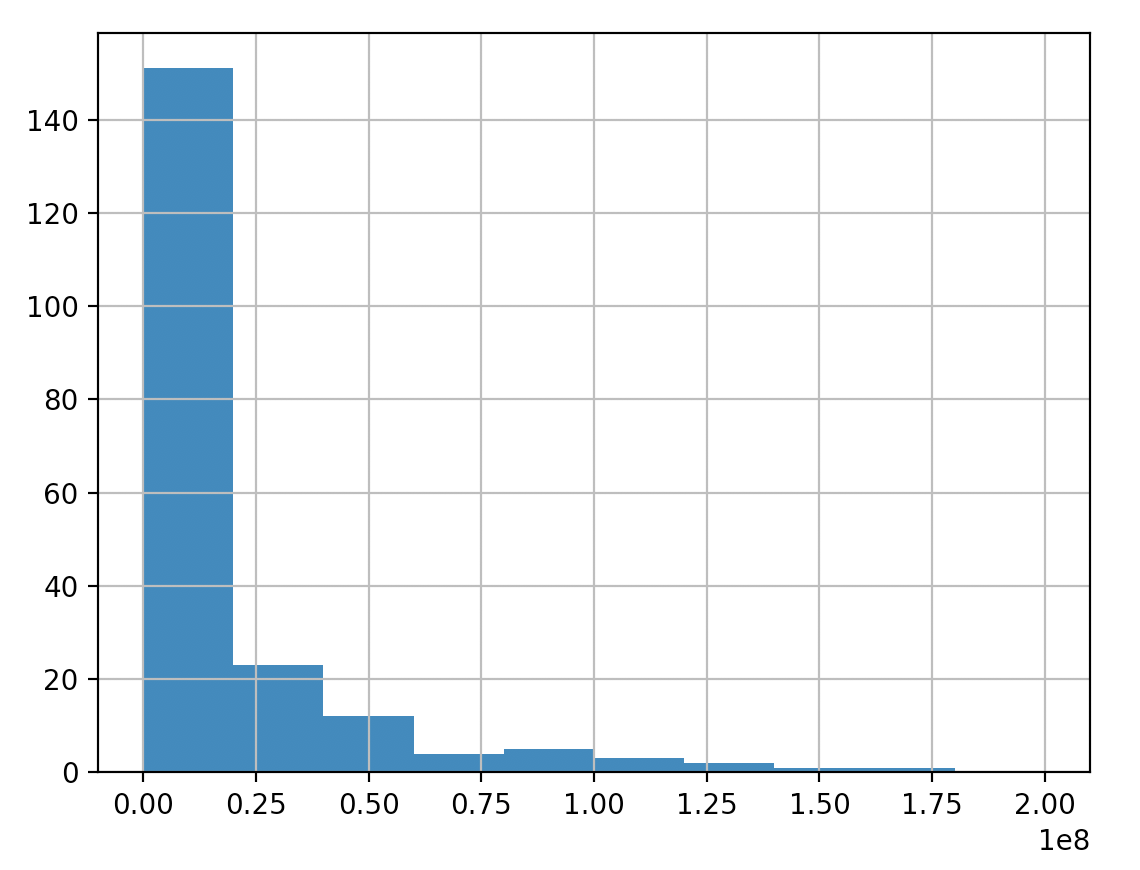
\includegraphics[scale=0.6]{fig/p3.png}
\end{center}
$\mu = 36694813.1722488$\\
$\sigma = 141822871.65179774$\\
About 150 out of 209 countries are in the first population bin. About 21 countries are in the second population bin. As
we go through the x-axis, the number of countries within the ranges remains low. The number of countries drops drastically
from the first bin to the second bin, which makes the distribution seems to be power-law distribution since very few countries contribute to a large
percent of populations and most countries have relatively small population size.

\section*{(4)}
\begin{lstlisting}
    mask = (df['dateRep'] == '2020-05-04')
    df2 = df.loc[mask]
    print(df2['cases'].median())
    q1 = df2['cases'].quantile(0.25)
    q3 = df2['cases'].quantile(0.75)
    print(q3 - q1)
    df2['cases'].hist(range = [0,10000])
    plt.show()
\end{lstlisting}
\begin{center}
    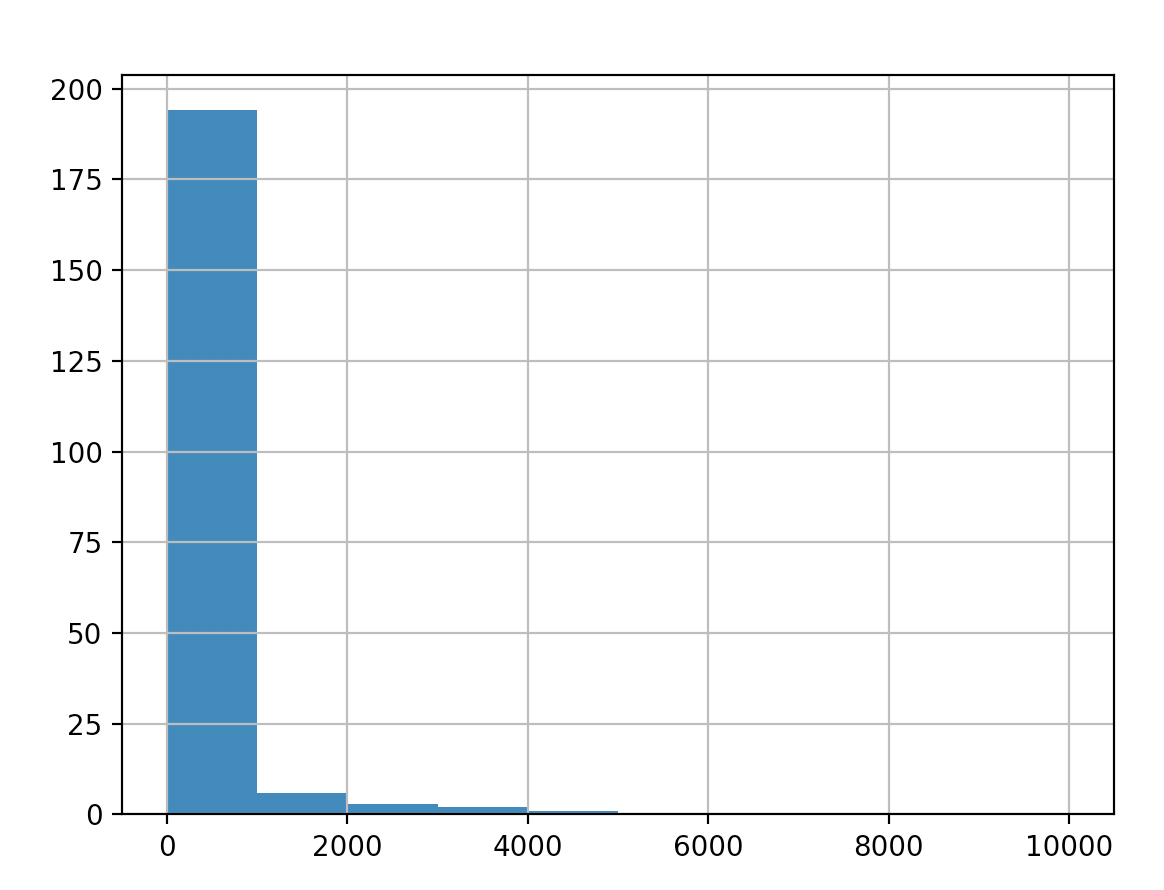
\includegraphics[scale=0.5]{fig/p4.png}
\end{center}
$Median = 5.0$\\
$IQR = Q_{3} - Q_{1} = 90.75 - 0.00 = 90.75$
About 190 out of 209 countries are in the first cases reported bin. As we go through the x-axis, the number of reported cases decreases drastically.
Since the first bin is significantly larger than the others, this distribution seems to be power-law distribution.

\section*{(5)}
\begin{lstlisting}
    mask = (df['dateRep'] >= '2020-06-01') & (df['dateRep'] <= '2020-07-01')
    df2 = df.loc[mask]
    df2 = df2[['countriesAndTerritories','cases']]
    df2 = df2.sort_values('cases',ascending=False)
    print(df2)
\end{lstlisting}
\textbf{Brazil} had the greatest increase in the number of cases from June 1st to July 1st. The increase is $54,771$.

\section*{(6)}
\begin{lstlisting}
    mask = (df['dateRep'] >= '2020-06-01') & (df['dateRep'] <= '2020-07-01')
    df2 = df.loc[mask]
    df2 = df2[['countriesAndTerritories','cases']]
    df2 = df2.groupby(['countriesAndTerritories']).sum()
    df2['cases'] = df2['cases']/31
    df2 = df2.sort_values('cases',ascending=False)
    print(df2)
\end{lstlisting}
\textbf{Brazil} had the greatest average increase in the number of cases per day from June 1st to July 1st. The average increase is $29148.419355$.

\section*{(7)}
\begin{lstlisting}
    mask = (df['dateRep'] >= '2020-06-01') & (df['dateRep'] <= '2020-07-01')
    df2 = df.loc[mask]
    df2 = df2[['countriesAndTerritories','cases','popData2019']]
    df2 = df2.groupby(['countriesAndTerritories','popData2019'],as_index=False).sum()
    df2["result"] = ""
    df2['result'] = df2['cases']/df2['popData2019']*10000
    df2 = df2.sort_values('result',ascending=False)
    print(df2)
\end{lstlisting}
\textbf{Qatar} had the greatest increase in average cases per 10,000 people per day from June 1st to July 1st. The average is $144.15599$.

\section*{(8)}
\begin{lstlisting}
    df2 = df[['dateRep','countriesAndTerritories','cases','deaths']]
    df2 = df2.groupby(['dateRep']).sum().sort_values('cases',ascending=False)
    print(df2)
\end{lstlisting}
On \textbf{July 30th, 2020}, the world had the greatest number of reported cases($298,094$ cases).
\begin{lstlisting}
    df2 = df2.sort_values('deaths',ascending=False)
    print(df2)
\end{lstlisting}
On \textbf{April 16th, 2020}, the world had the greatest number of reported deaths($10,542$ cases).


\section*{(9)}

\begin{lstlisting}
df_holder = (df['dateRep'] >= '2020-06-01') & (df['dateRep'] <= '2020-08-01')
df_holder = df.loc[df_holder]
df_holder = df_holder[['dateRep','countriesAndTerritories','cases','deaths']]
df_us_case = df_holder.loc[df['countriesAndTerritories'] == 'United_States_of_America']

df_us_case.plot(x = 'dateRep', y = ['deaths', 'cases'])
plt.show()
\end{lstlisting}

\begin{center}
    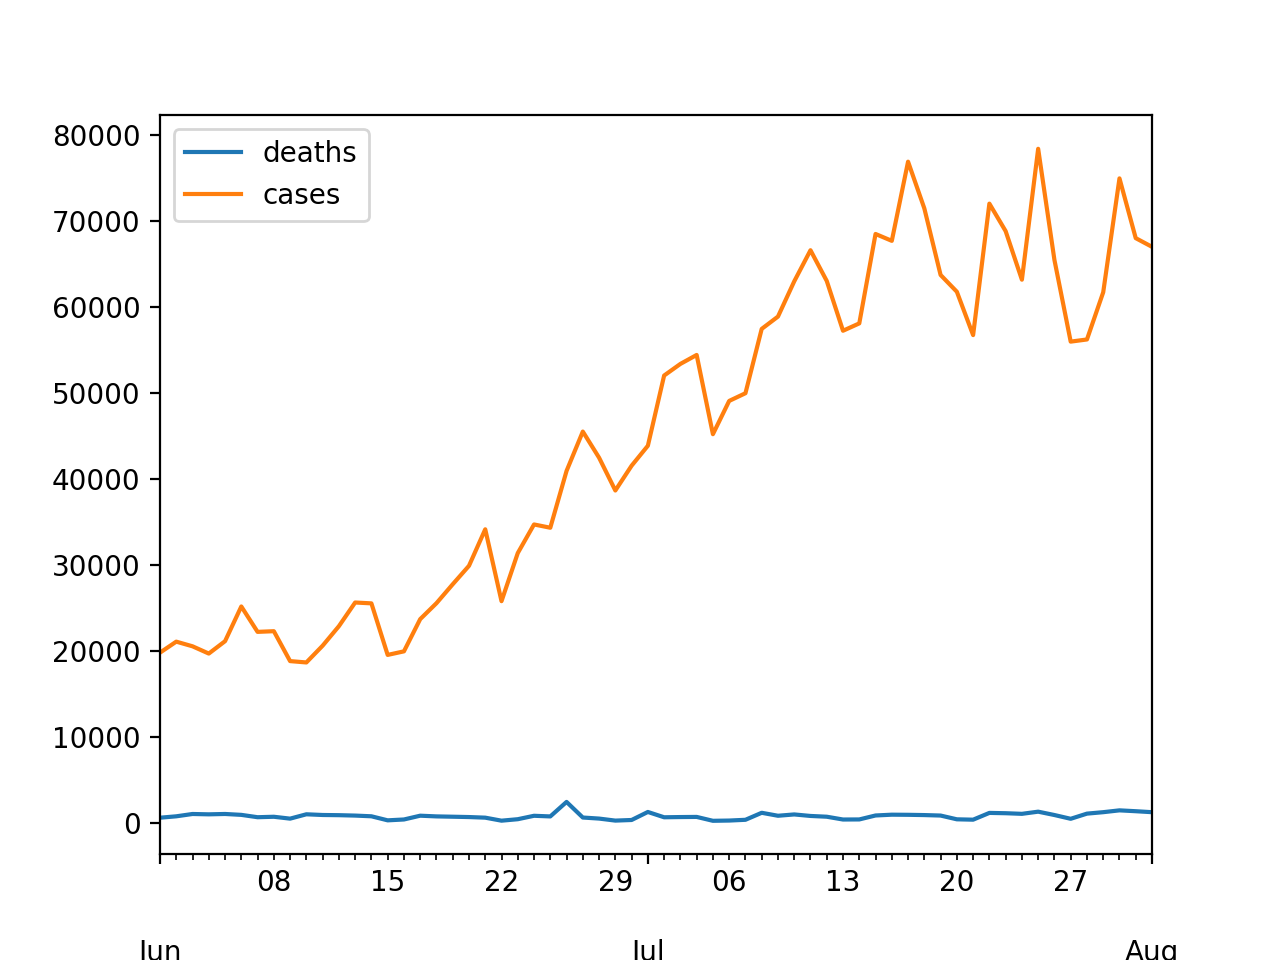
\includegraphics[scale=0.5]{fig/p9.png}
\end{center}

It seems depite the significant increase on daily new cases, the amount of deaths -- altough still sad to say -- is actually rather steady on the graph. Which our first thought is the large \ilc{Y}-axis scale on \ilc{cases} makes growth of \ilc{deaths} hardly noticeable, but with close examination it is actually not the case. Thus, our guess it is that during June to Augest, the pressure on US medical system is not as hard, so that health care works can actually ``control'' the death of COVID-19 to a certain extent.




\end{document}